\documentclass[12pt,conference]{IEEEtran}
\IEEEoverridecommandlockouts
% The preceding line is only needed to identify funding in the first footnote. If that is unneeded, please comment it out.
\usepackage{cite}
\usepackage{amsmath,amssymb,amsfonts}
\usepackage{algorithmic}
\usepackage{graphicx}
\usepackage{textcomp}
\usepackage{xcolor}
\usepackage{hyperref}
\usepackage{listings}

\lstset{
    basicstyle=\small\ttfamily,
    columns=flexible,
    breaklines=true
}

\def\BibTeX{{\rm B\kern-.05em{\sc i\kern-.025em b}\kern-.08em
    T\kern-.1667em\lower.7ex\hbox{E}\kern-.125emX}}

\begin{document}

\title{\{Insert Title Here\}: Fine-tuning a language model to predict titles\\
}

\author{\IEEEauthorblockN{1\textsuperscript{st} Louis Stanko}
\textit{Ludwig-Maximilians-Universitaet}\\
\\
Munich, Germany \\
l.stanko@campus.lmu.de}
}

\maketitle

\begin{abstract}

This paper presents a partial replication study of "Can Pre-Trained Language Models Generate Titles for Research Papers?" Instead of fine-tuning large or medium-scale transformer models, I investigate whether a 135-million parameter model, called SmolLM-135M, can achieve competitive title generation performance. I experiment with both full fine-tuning (FFT) and Low-Rank Adaptation (LoRA) across two training regimes: a small domain-specific dataset (CSPubSum) and a larger, more diverse dataset comprising over 2.4 million samples drawn from arXiv, Wikipedia, and Medium blog articles. Evaluation is performed on the LREC-COLING 2024 benchmark using ROUGE-1, ROUGE-2, and ROUGE-L scores. My best configuration, full fine-tuning on the large dataset, achieves ROUGE-1/2/L scores of 41.32/22.51/35.21, approaching the performance of fine-tuned large language models at a fraction of the parameter count. In the following, I discuss training dynamics, the effect of dataset scale, and the impact of generation length on evaluation scores. Last but not least, the final model is converted to ONNX format and deployed as a browser-based application using Transformers.js.

%{'loss': 11.6742, 'grad_norm': 1.7175283432006836, 'learning_rate': 3.841897233201582e-05, 'epoch': 0.2}            
% {'loss': 11.0562, 'grad_norm': 2.64554762840271, 'learning_rate': 3.6837944664031623e-05, 'epoch': 0.39}            
% {'loss': 10.0484, 'grad_norm': 2.647836446762085, 'learning_rate': 3.525691699604744e-05, 'epoch': 0.59}            
% {'loss': 8.8266, 'grad_norm': 3.662590265274048, 'learning_rate': 3.3675889328063244e-05, 'epoch': 0.79}            
% {'loss': 7.3205, 'grad_norm': 6.181723117828369, 'learning_rate': 3.209486166007906e-05, 'epoch': 0.99}             
% {'loss': 5.6689, 'grad_norm': 4.24257755279541, 'learning_rate': 3.0513833992094867e-05, 'epoch': 1.18}             
% {'loss': 3.8653, 'grad_norm': 4.670482158660889, 'learning_rate': 2.8932806324110677e-05, 'epoch': 1.38}            
% {'loss': 1.9127, 'grad_norm': 3.34485125541687, 'learning_rate': 2.7351778656126488e-05, 'epoch': 1.58}             
% {'loss': 0.5358, 'grad_norm': 0.43193256855010986, 'learning_rate': 2.5770750988142298e-05, 'epoch': 1.77}
% {'loss': 0.2925, 'grad_norm': 0.16923046112060547, 'learning_rate': 2.4189723320158104e-05, 'epoch': 1.97}
% {'loss': 0.2716, 'grad_norm': 0.18348507583141327, 'learning_rate': 2.2608695652173914e-05, 'epoch': 2.17}
% {'loss': 0.25, 'grad_norm': 0.08930478245019913, 'learning_rate': 2.1027667984189725e-05, 'epoch': 2.36}
% {'loss': 0.2594, 'grad_norm': 0.13114279508590698, 'learning_rate': 1.9446640316205535e-05, 'epoch': 2.56}
% {'loss': 0.2497, 'grad_norm': 0.07828853279352188, 'learning_rate': 1.7865612648221345e-05, 'epoch': 2.76}
% {'loss': 0.2465, 'grad_norm': 0.1263086497783661, 'learning_rate': 1.6284584980237155e-05, 'epoch': 2.96}
% {'loss': 0.2495, 'grad_norm': 0.13955603539943695, 'learning_rate': 1.4735177865612648e-05, 'epoch': 3.15}
% {'loss': 0.2386, 'grad_norm': 0.0754985362291336, 'learning_rate': 1.3154150197628458e-05, 'epoch': 3.35}
% {'loss': 0.2225, 'grad_norm': 0.06165948510169983, 'learning_rate': 1.157312252964427e-05, 'epoch': 3.55}
% {'loss': 0.2304, 'grad_norm': 0.29593583941459656, 'learning_rate': 9.99209486166008e-06, 'epoch': 3.74}
% {'loss': 0.2417, 'grad_norm': 0.08827625215053558, 'learning_rate': 8.41106719367589e-06, 'epoch': 3.94}
% {'loss': 0.2393, 'grad_norm': 0.07319273799657822, 'learning_rate': 6.830039525691701e-06, 'epoch': 4.14}

% New one, trained correctly on CSPubSum..
% {'train_runtime': 915.3711, 'train_samples_per_second': 44.354, 'train_steps_per_second': 1.382, 'train_loss': 2.9474008673264573, 'epoch': 4.99}
% {'loss': 2.9242, 'grad_norm': 0.05597302317619324, 'learning_rate': 5.2173913043478265e-06, 'epoch': 4.33}                                              
% {'loss': 2.9191, 'grad_norm': 0.059621382504701614, 'learning_rate': 2.0553359683794467e-06, 'epoch': 4.73}
% {'loss': 2.923, 'grad_norm': 0.0632089227437973, 'learning_rate': 1.1541501976284585e-05, 'epoch': 3.55}  
% {'loss': 2.9229, 'grad_norm': 0.059308744966983795, 'learning_rate': 8.379446640316207e-06, 'epoch': 3.94}
% {'loss': 2.9298, 'grad_norm': 0.061494581401348114, 'learning_rate': 1.7865612648221345e-05, 'epoch': 2.76}
% {'loss': 2.921, 'grad_norm': 0.05799975246191025, 'learning_rate': 1.4703557312252965e-05, 'epoch': 3.15}
% {'loss': 2.9464, 'grad_norm': 0.05599372088909149, 'learning_rate': 2.4189723320158104e-05, 'epoch': 1.97}
% {'loss': 2.9346, 'grad_norm': 0.05538400635123253, 'learning_rate': 2.1027667984189725e-05, 'epoch': 2.36}
% {'loss': 2.963, 'grad_norm': 0.05159113183617592, 'learning_rate': 3.0513833992094867e-05, 'epoch': 1.18}
% {'loss': 2.9557, 'grad_norm': 0.058177486062049866, 'learning_rate': 2.7351778656126488e-05, 'epoch': 1.58}
% {'loss': 3.0366, 'grad_norm': 0.05678539350628853, 'learning_rate': 3.6837944664031623e-05, 'epoch': 0.39}
% {'loss': 3.008, 'grad_norm': 0.05907018855214119, 'learning_rate': 3.3675889328063244e-05, 'epoch': 0.79}

% New dataset with 2.6m samples:
% {'loss': 2.9796, 'grad_norm': 0.0759323462843895, 'learning_rate': 3.9990511433722366e-05, 'epoch': 0.0}
% {'loss': 2.9292, 'grad_norm': 0.0721476674079895, 'learning_rate': 3.998102286744473e-05, 'epoch': 0.0}
% {'loss': 2.8117, 'grad_norm': 0.06756923347711563, 'learning_rate': 3.981971724072493e-05, 'epoch': 0.02}
% {'loss': 2.7846, 'grad_norm': 0.07364869117736816, 'learning_rate': 3.9734415029888985e-05, 'epoch': 0.03}
% {'loss': 2.7842, 'grad_norm': 0.08605469763278961, 'learning_rate': 3.966799506594554e-05, 'epoch': 0.04}
% {'loss': 2.7926, 'grad_norm': 0.06697369366884232, 'learning_rate': 3.9630040800835e-05, 'epoch': 0.05}
% {'loss': 2.7965, 'grad_norm': 0.07750755548477173, 'learning_rate': 3.9573109403169184e-05, 'epoch': 0.05}
% {'loss': 2.7757, 'grad_norm': 0.08127438277006149, 'learning_rate': 3.862434766106842e-05, 'epoch': 0.17}
% {'loss': 2.7757, 'grad_norm': 0.08135705441236496, 'learning_rate': 3.862434766106842e-05, 'epoch': 0.17}
% {'loss': 2.7771, 'grad_norm': 0.1169646605849266, 'learning_rate': 3.851048486573679e-05, 'epoch': 0.19}
% {'loss': 2.7843, 'grad_norm': 0.09231168031692505, 'learning_rate': 3.838713350412753e-05, 'epoch': 0.2}
% {'loss': 2.7605, 'grad_norm': 0.08332296460866928, 'learning_rate': 3.833969067273935e-05, 'epoch': 0.21}
% {'loss': 2.7758, 'grad_norm': 0.09091147035360336, 'learning_rate': 3.801622159124945e-05, 'epoch': 0.25}
\end{abstract}

\begin{IEEEkeywords}
SmolLM-135M, fine-tuning, title generation
\end{IEEEkeywords}

\section{Introduction}
Automatic title generation for scientific papers is a fairly well-studied sequence-to-sequence task with broad practical applications like academic search, recommendation systems, or mobile apps like calendars or To-do apps. A well-formed title should be concise, informative, and factually grounded in the source. At the same time, it is constrained to a relatively short output, typically under 20 tokens, which raises an interesting question: does effective title generation actually require a large language model?
The reference paper by Rehman et al. \cite{b2}, "Can Pre-Trained Language Models Generate Titles for Research Papers?", explores this using the models: T5-base, BART-base, PEGASUS-large, LLaMA-3-8B, and GPT-3.5-turbo on the LREC-COLING 2024 benchmarks. However, the study does not examine the low end of the model size spectrum.

Motivated by the hypothesis that title generation is a relatively constrained task that may not require large-scale parametric capacity, this work investigates SmolLM-135M, a decoder-only causal language model with only 135 million parameters. I conduct experiments across two fine-tuning strategies (full fine-tuning and LoRA) and two dataset regimes (domain-specific and large-scale diverse), and report results on the LREC-COLING 2024 test set. The LREC-COLING 2024 dataset was introduced in the reference paper by Rehman et al. \cite{b2}. The goal is not to achieve state-of-the-art performance, but to understand how far a small, efficiently deployable model can go, and to identify the conditions under which it succeeds or fails.

As a secondary contribution, I demonstrate practical deployment: the best model is exported to ONNX format and served entirely in the browser via Transformers.js, illustrating that research-quality title generation can run locally without any server infrastructure.

\section{Related Work}
Title generation has historically been treated as a summarization problem, where the abstract plays the role of the source document and the title is the extreme summary. Early work used extractive approaches and template-based methods. With the rise of neural sequence-to-sequence models, abstractive generation became dominant, with LSTM-based encoder-decoders eventually giving way to transformer architectures \cite{b1}.

The reference paper by Rehman et al. \cite{b2} is the most directly relevant work. They benchmark both encoder-decoder models and decoder-only LLMs on CSPubSum and LREC-COLING 2024, finding that fine-tuned T5-base and BART-base yield ROUGE-1 scores around 46--47 percent, while PEGASUS-large reaches nearly 50\%. Notably, the non-fine-tuned LLaMA-3-8B model in a zero-shot setting scores only 32.92 on ROUGE-1, highlighting the importance of task-specific fine-tuning even for large models.

LoRA \cite{b3} has emerged as an efficient alternative to full fine-tuning by injecting trainable low-rank matrices into frozen transformer layers. Rather than updating all model weights, LoRA introduces a small number of additional parameters (controlled by rank r) that are sufficient to adapt the model to new tasks. This significantly reduces memory and compute requirements, making it well-suited for consumer hardware.

SmolLM \cite{b4} is a family of compact causal language models trained on the SmolLM-Corpus, which includes curated web text and code. The 135M variant, used in this work, uses the MobileLLM \cite{b5} architecture and cosmo2-tokenizer\cite{b6}, making it compatible with standard HuggingFace tooling. To my knowledge, no prior work has evaluated SmolLM-135M on title generation.


\section{Data}

\subsection{Training Datasets}
I used two distinct training corpora representing different scales and domains.

\textbf{CSPubSum}: The CSPubSum training dataset contains 8,120 abstract-title pairs from computer science publications. This dataset was used in the original reference paper and represents the primary in-domain training resource for scientific title generation. Cleaning follows the same protocol as the reference paper: title length is constrained to between 3 and 20 tokens, and abstracts must be at least 20 tokens long. This requirement is necessary, in order to treat the title generation as an extreme form of text summarization.

\textbf{Large (diverse) Dataset}: To test whether broader training signal can compensate for domain mismatch, I construct a second training corpus by combining three sources: (1) a Kaggle dataset merging arXiv abstracts with Wikipedia articles, totaling approximately 2.65 million entries; (2) the Medium Articles dataset from Kaggle, containing approximately 192,000 blog posts with titles. The two sources are concatenated and subjected to a shared cleaning pipeline. 
\textbf{Note:} In the following this dataset is referred to as \textit{Large Dataset} or \textit{Large Diverse Dataset}. In the python code, this is usually referred to as \textit{own} or \textit{train\_data.csv}.


\begin{table}[h]
\centering
\caption{Datasets Used}
\begin{tabular}{ll}
\hline
\textbf{Name} & \textbf{Samples} \\
\hline
\href{https://www.kaggle.com/datasets/monikaavagyan/combined-dataset-from-arxiv-and-wikipedia}{Wikipedia} & 900{,}000 \\
\href{https://www.kaggle.com/datasets/fabiochiusano/medium-articles}{Medium.com} & 190{,}000 \\
\href{https://www.kaggle.com/datasets/Cornell-University/arxiv}{Arxiv} & 1{,}750{,}000 \\
\hline
\end{tabular}
\end{table}

\subsection{Data Cleaning}

Both datasets pass through the following cleaning steps. First, duplicates are removed. Second, samples with titles containing LaTeX mathematical expressions (e.g., dollar-sign delimited formulas), numbers greater than 99, or parenthetical expressions are filtered out, as these tend to produce noisy or unpredictable targets. Third, all samples are tokenized using the cosmos2 tokenizer, and only those where the concatenated text (abstract + title prompt) fits within 512 tokens are retained. Finally, any samples whose titles appear in the LREC-COLING 2024 \textbf{test set} are removed to prevent data leakage.

\begin{figure}[htbp]
\centering
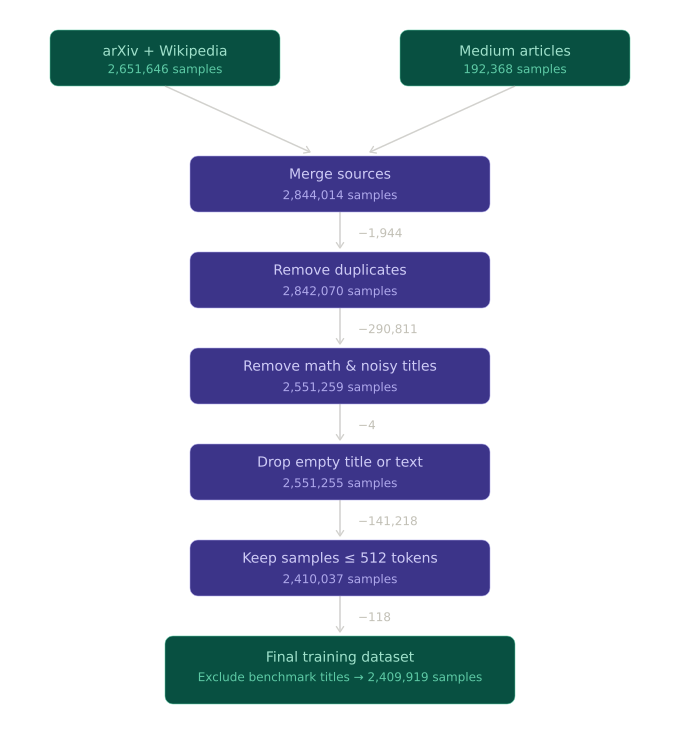
\includegraphics[width=1\columnwidth]{data_cleaning_pipeline(1).png}
\caption{Visualization of data cleaning pipeline for the large diverse dataset.}
\label{fig:dataCleaning}
\end{figure}

After cleaning, the large dataset contains approximately 2.41 million samples. A notable consequence of the LaTeX filtering is the removal of a substantial fraction of arXiv papers, many of which contain mathematical notation in their titles. This may shift the distribution of the large dataset toward more general-domain content, which may explain some of the generalisation patterns observed in the results. See Figure \ref{fig:dataCleaning} for a detailed breakdown of the cleaning pipeline.

\subsection{Evaluation Dataset}

All models are evaluated on the LREC-COLING 2024 test set, a benchmark of scientific paper title-abstract pairs released alongside the reference paper. As an effort to make my results easier to reproduce, I published the test set on Kaggle \cite{b7}. This set is held out from all training data, as described above.

\section{Methodology}

\subsection{Base Model}
All experiments use SmolLM-135M v1 (\href{https://huggingface.co/HuggingFaceTB/SmolLM-135M}{HuggingFaceTB/SmolLM-135M}) as the base model. This is a decoder-only causal language model with 135 million parameters, trained on a mixture of web text and code. It uses the cosmos2-tokenizer in conjunction with a vocabulary of size 49{,}152. The model is publicly available on HuggingFace \cite{b8}. For more information about the architecture and hyper-parameters used, visit \href{https://huggingface.co/blog/smollm}{https://huggingface.co/blog/smollm}.

I decided to use the first version of the SmolLM-135M model, as the successor only yielded small improvements over the first version. Additionally, the first version was released in February 2024, which is close to the release date of the reference paper (September 2024), allowing for a fairer comparison.

\subsection{Prompt Format}
I frame title generation as a conditional language modeling task. Each training example is formatted as:

\texttt{<abstract>\textbackslash{n}\textbackslash{n}Title: <title><EOS>}

During inference, only the abstract and the "Title:" prompt are provided, and the model generates the title autoregressively. Loss is computed only on the title tokens (the abstract prefix is masked with -100 labels in the full fine-tuning setup). This causal language modeling approach is standard for decoder-only models adapted to generation tasks. When fine-tuning LoRA, no masking was done and the loss was computed on the entire input sequence. This was due to a lack of understanding. Unfortunately, this could have had a negative impact on fine-tuning, as the model gets rewarded to memorize the entire input sequence rather than just focusing on the title. 

\subsection{LoRA Fine-Tuning}
The first experimental setup uses Low-Rank Adaptation (LoRA). LoRA is applied with rank ($r$) = 16, alpha ($\alpha$) = 16, and dropout of 0.05, targeting the default query and value projection layers. Since $r==\alpha$, the \textbf{effective adaptation strength} ($\frac{r}{\alpha}) = 1$, implying a stable adjustment of weight changes. As $\alpha$ denotes the "impact" of the update which is applied to the weights and $r$ The model is trained on the large diverse dataset for 5 epochs using the SFTTrainer. Batch size is 8 with 4 gradient accumulation steps (effective batch size 32), and learning rate is 4e-5 (0,00004). These metrics were taken from the reference paper, but are also considered “sane defaults” in the machine learning community. The SFTTrainer (supervised fine-tuning) operates on raw formatted text strings rather than pre-tokenized sequences, using the text field from the formatted examples, however, during cleaning the actual input size was already measured in tokens. \\

Also relevant for the LoRA configuration, is that the base model contains eight distinct linear layer types: \texttt{q\_proj, k\_proj, v\_proj, o\_proj, gate\_proj, up\_proj, down\_proj}, and \texttt{lm\_head}. By default, the python library used for this experiment, huggingface PEFT \cite{b9}, adjusts only \texttt{q\_proj} and \texttt{v\_proj}. I adopt this default in the experiments due to computation and time constraints. 
Nevertheless, I would encourage further experiments which adapt more linear layers as these would likely boost accuracy. 

Another observation which is worth mentioning that these settings reduce the size from 135 million (135,436,608 to be exact) parameters to 921,600. That is 0.68\% of all tunable parameters and might help explain some of the results in the later sections. 

The fine-tuning happened on an NVIDIA V100 16GB VRAM GPU node hosted in the LRZ cloud. Training on the large dataset took 100 hours.

After training, the LoRA adapter is merged into the base model weights, which produces a standard HuggingFace model that can be distributed independently.

\subsection{Full Fine Tuning (FFT)}
In the second experimental setup, all model weights are updated during training. I conduct two FFT runs: one on the small CSPubSum dataset and one on the large diverse dataset.

For the CSPubSum run, training proceeds for 1 epoch using a batch size of 16 with 2 gradient accumulation steps (effective batch size 32), an unchanged learning rate of 4e-5 with a cosine scheduler and 3\% warmup ratio. For the large dataset run, the same hyperparameters are used but training is capped at 1 epoch due to the dataset size and insights from the previous fine tuning run, where after the first epoch a validation plateau was reached.

The fine-tuning happened on an NVIDIA V100 16GB VRAM GPU node hosted in the LRZ cloud. Training took 10 hours.

\subsection{Evaluation}
Title generation is performed with greedy decoding (\texttt{do\_sample=False}, for repeatability) and a maximum of 30 new tokens. The 30-token limit was selected based on empirical observation: using 20 tokens produced significantly worse scores (approximately 20\% ROUGE-1 degradation). An investigation (Figure~\ref{fig:TitleTokenDistribution}) revealed that, although the distribution of title token lengths has a mean of 15.27 tokens, it exhibits a right tail, with a non-trivial portion of titles exceeding 20 tokens. When generation is capped at 20 tokens, these longer titles are forcibly truncated before completion. This causes the model to output partial titles that fail to match their full references during ROUGE evaluation. A truncated output structurally cannot recover the tokens it never produced, negatively impacting recall and the F1 score. Extending the limit to 30 tokens covers the overwhelming majority of the distribution, allowing nearly all titles to be generated in full. 

\begin{figure}[htbp]
\centering
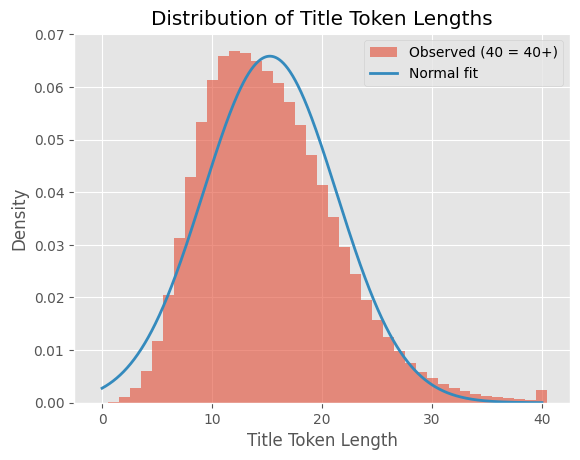
\includegraphics[width=\columnwidth]{title-token-distribution.png}
\caption{Average Title Token Distribution. }
\label{fig:TitleTokenDistribution}
\end{figure}

\subsection{Evaluation Metrics}

To make my results comparable a widely accepted baseline called ROUGE is used. ROUGE stands for Recall-Oriented Understudy for Gisting Evaluation, and can be measured in different ways. I report F1 scores for ROUGE-1, ROUGE-2, and ROUGE-L using the rouge-score python library with stemming enabled \cite{b11}.  ROUGE-1/2 are part of the ROUGE-N family which measures the $n$-gram between a \textit{hypothesis} (the generated title) and the \textit{ground-truth} (the actual title). An $n$-gram is a sequence of $n$ adjacent symbols in a particular order. For example, Table~\ref{tab:ngram_example} illustrates how a sentence is decomposed into 1-grams and 2-grams.

\begin{table}[htbp]
\centering
\caption{Example of $n$-gram extraction from a sample sequence}
\begin{tabular}{|p{2.2cm}|p{2.5cm}|p{3.1cm}|}
\hline
\textbf{Example} & \textbf{1-gram sequence} & \textbf{2-gram sequence} \\ \hline
... to be or not ... & 
... to, be, or, not, ... & 
... to be, be or, or not, ... \\ \hline
\end{tabular}
\label{tab:ngram_example}
\end{table}

ROUGE-L, simply measures the longest common subsequence (LCS) in both, the hypothesis and the ground-truth. A subsequence is a string generated from the ground-truth by deleting 0 or more characters, without changing the relative order of the remaining characters.

Last but not least, stemming is a preprocessing technique that reduces words to their word stems by removing suffixes and prefixes (e.g. run\textbf{s} $\rightarrow$ run \& run\textbf{ning} $\rightarrow$ run). This might be a deviation from the reference paper, unfortunately, I was unable to find any artifacts of the code used for evaluating Rehman et al. \cite{b2} fine-tuned models.


% From Batch 19200, we employed logging and a validation of 1\% of the total dataset size.
% There 

\section{Results}

ROUGE scores are computed against lowercased and stemmed ground-truth titles using F1 measures for ROUGE-1, ROUGE-2, and ROUGE-L.

Additionally, entity-level factual consistency metrics (precision, recall, F1 over named entities extracted using SciSpacy) are also computed in the evaluation script, following the methodology of the reference paper, though, in the following, I focus on ROUGE as the primary comparison metric due to required brevity. 

The results of the factual consistency score can be found in the appendix \ref{fig:FactualOwn}.

\begin{figure}[htbp]
\centering
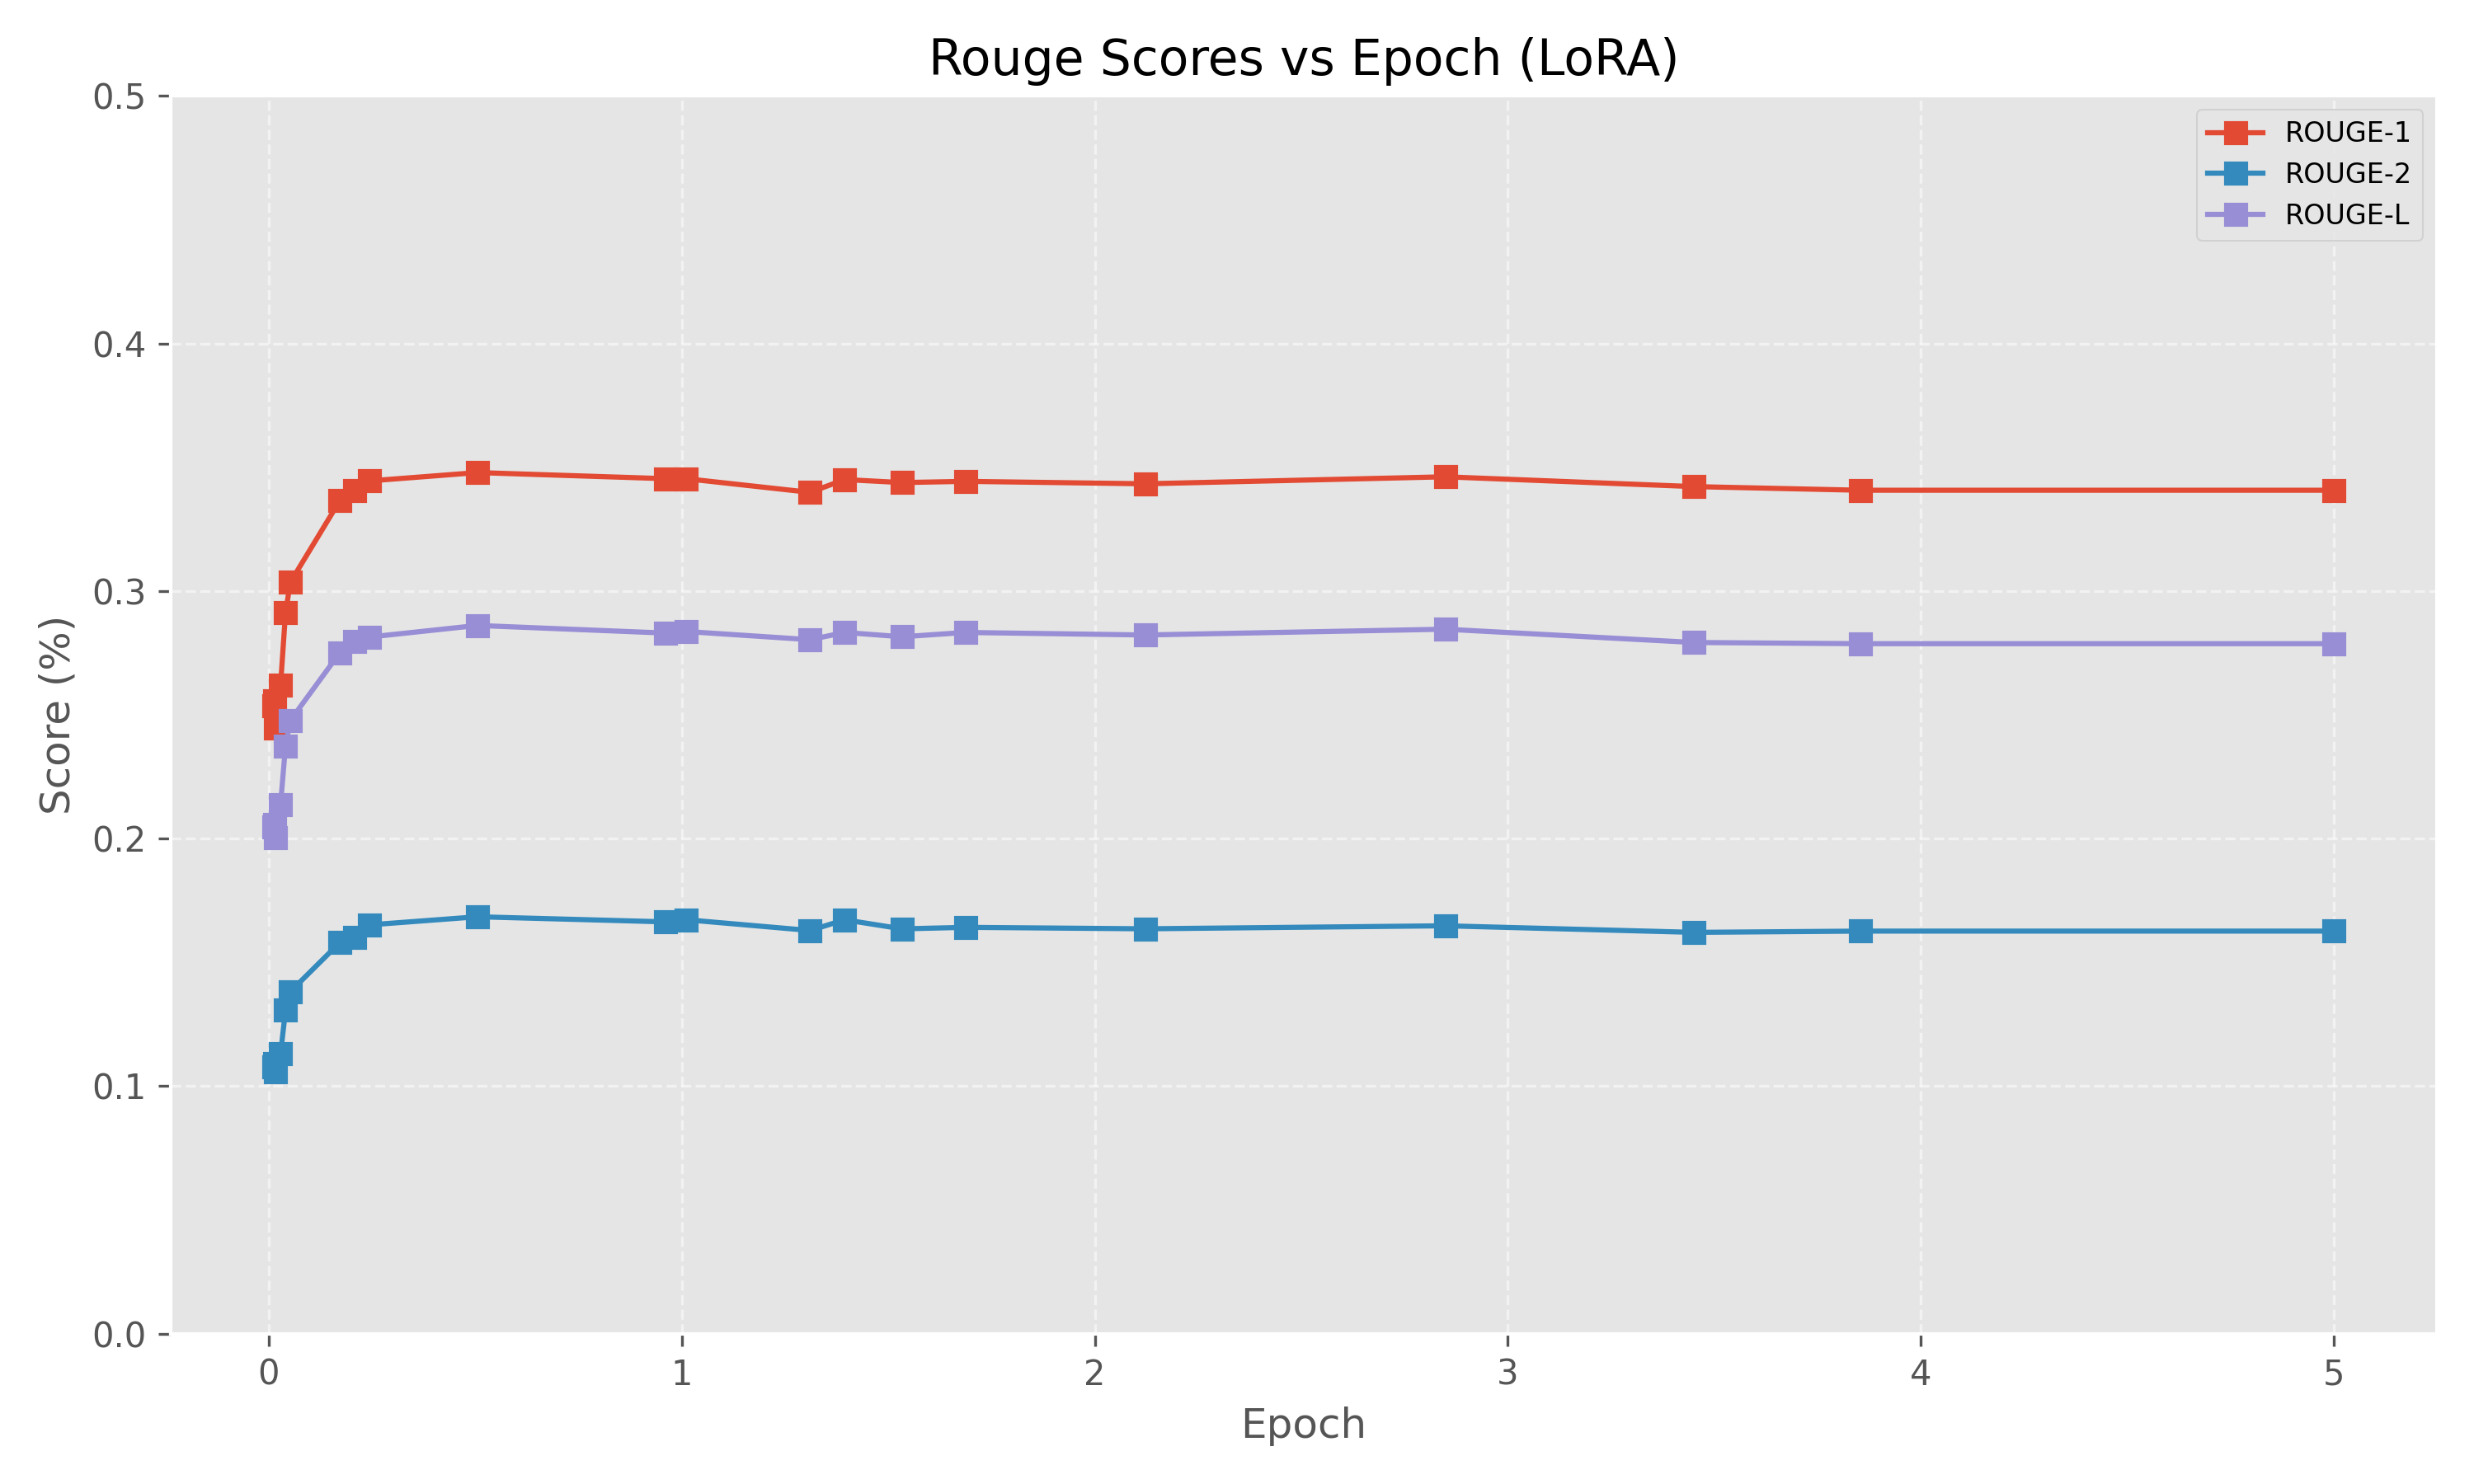
\includegraphics[width=\columnwidth]{rouge_own.png}
\caption{ROUGE scores of \textbf{Large Dataset} when fine-tuning using LoRA for 5 epochs. The validation set was LREC-COLING 2024.}
\label{fig:RougeOwn}
\end{figure}

During the first half of the first epoch, rouge scores increase dramatically. From $\approx$~25\% to $\approx$~34\% for ROUGE-1, which is a $40\%$ increase! 
For the rest of the fine-tuning, performance hits a plateau. For ROUGE-1 that is at around 33\%. ROUGE-2 and ROUGE-L hover around 16\% and 28\% respectively. The graph is capped at 50\%, to show the ROUGE-1 score of the best performing model from the reference paper, PEGASUS-large.

The best recorded checkpoint was after 42200 steps. 5 epochs were 417345 steps and took 100 hours walltime. In hind-sight, fine-tuning could have been stopped after $\approx$~10~hours. However, validation was done after the fine-tuning finished, revealing this pattern too late. \\

Table \ref{tab:rouge_comparison} presents the measurements from the best checkpoint across all experimental configurations alongside the measurements from the reference paper. Our own results are highlighted in bold.

\begin{table}[htbp]
\caption{ROUGE-1/2/L F1 scores on the LREC-COLING 2024 test set. Reference results from Rehman  et al. \cite{b2}. Results in bold.}
\begin{center}
\begin{tabular}{|l|c|c|c|}
\hline
\textbf{Model} & \multicolumn{3}{|c|}{\textbf{ROUGE Metrics}} \\
\cline{2-4}
 & \textbf{\textit{1}} & \textbf{\textit{2}} & \textbf{\textit{L}} \\
\hline
T5-base                      & 46.84 & 28.70 & 41.69 \\
BART-base                    & 46.87 & 27.66 & 41.89 \\
PEGASUS-large                & 49.85 & 30.51 & 43.93 \\
LLaMA-3-8B zero-shot         & 32.92 & 16.66 & 27.66 \\
LLaMA-3-8B fine-tuned        & 45.30 & 26.53 & 40.51 \\
GPT-3.5-turbo                & 45.16 & 23.97 & 38.88 \\
\hline
\textbf{SmolLM LoRA CSPubSum}    & 25.52 & 10.90 & 20.54 \\
\textbf{SmolLM FFT CSPubSum}     & 35.36 & 17.54 & 30.12 \\
\textbf{SmolLM LoRA Large Dataset} & 34.79 & 16.84 & 28.61 \\
\textbf{SmolLM FFT Large Dataset}  & 41.32 & 22.51 & 35.21 \\
\hline
\multicolumn{4}{l}{$^{\mathrm{a}}$ ROUGE scores reported as percentages.}
\end{tabular}
\label{tab:rouge_comparison}
\end{center}
\end{table}

One can see, the FFT model trained exclusively on CSPubSum (8,120 samples) achieves ROUGE-1/2/L of 35.36/17.54/30.12. While this is below almost all reference models, it is notable that a 135M parameter model fine-tuned on fewer than 10,000 samples produces non-trivial scores at all, suggesting the task is learnable even with minimal data.

The LoRA model trained on the same CSPubSum dataset achieves lower scores of 25.52/10.90/20.54. This is likely due to the fact that the base model lacked exposure to scientific corpora during pre-training. Therefore, the restricted parameter space of the adapters cannot effectively synthesize the necessary domain-specific knowledge.

In contrast, the LoRA model trained on the large diverse dataset for 5 epochs achieves 34.79 / 16.84 / 28.61, a slight regression from the CSPubSum FFT baseline. This is likely due to the limited representational flexibility of low rank adaption. Here, scientific summarization could simply be too complex and benefit from deeper model adaption.
% The LoRA approach benefits from the broader distribution of the large training corpus while keeping the number of trainable parameters low.

The strongest result is achieved by the FFT model trained on the large diverse dataset: 41.32/22.51/35.21. This is competitive with the zero-shot LLaMA-3-8B baseline (32.92/16.66/27.66) and comes close to models that are 60 times larger. The gap to the best reference model (PEGASUS-large: 49.85/30.51/43.93) remains substantial, but the result illustrates that a 135M model with appropriate training data can perform surprisingly well.

\begin{figure}[htbp]
\centering
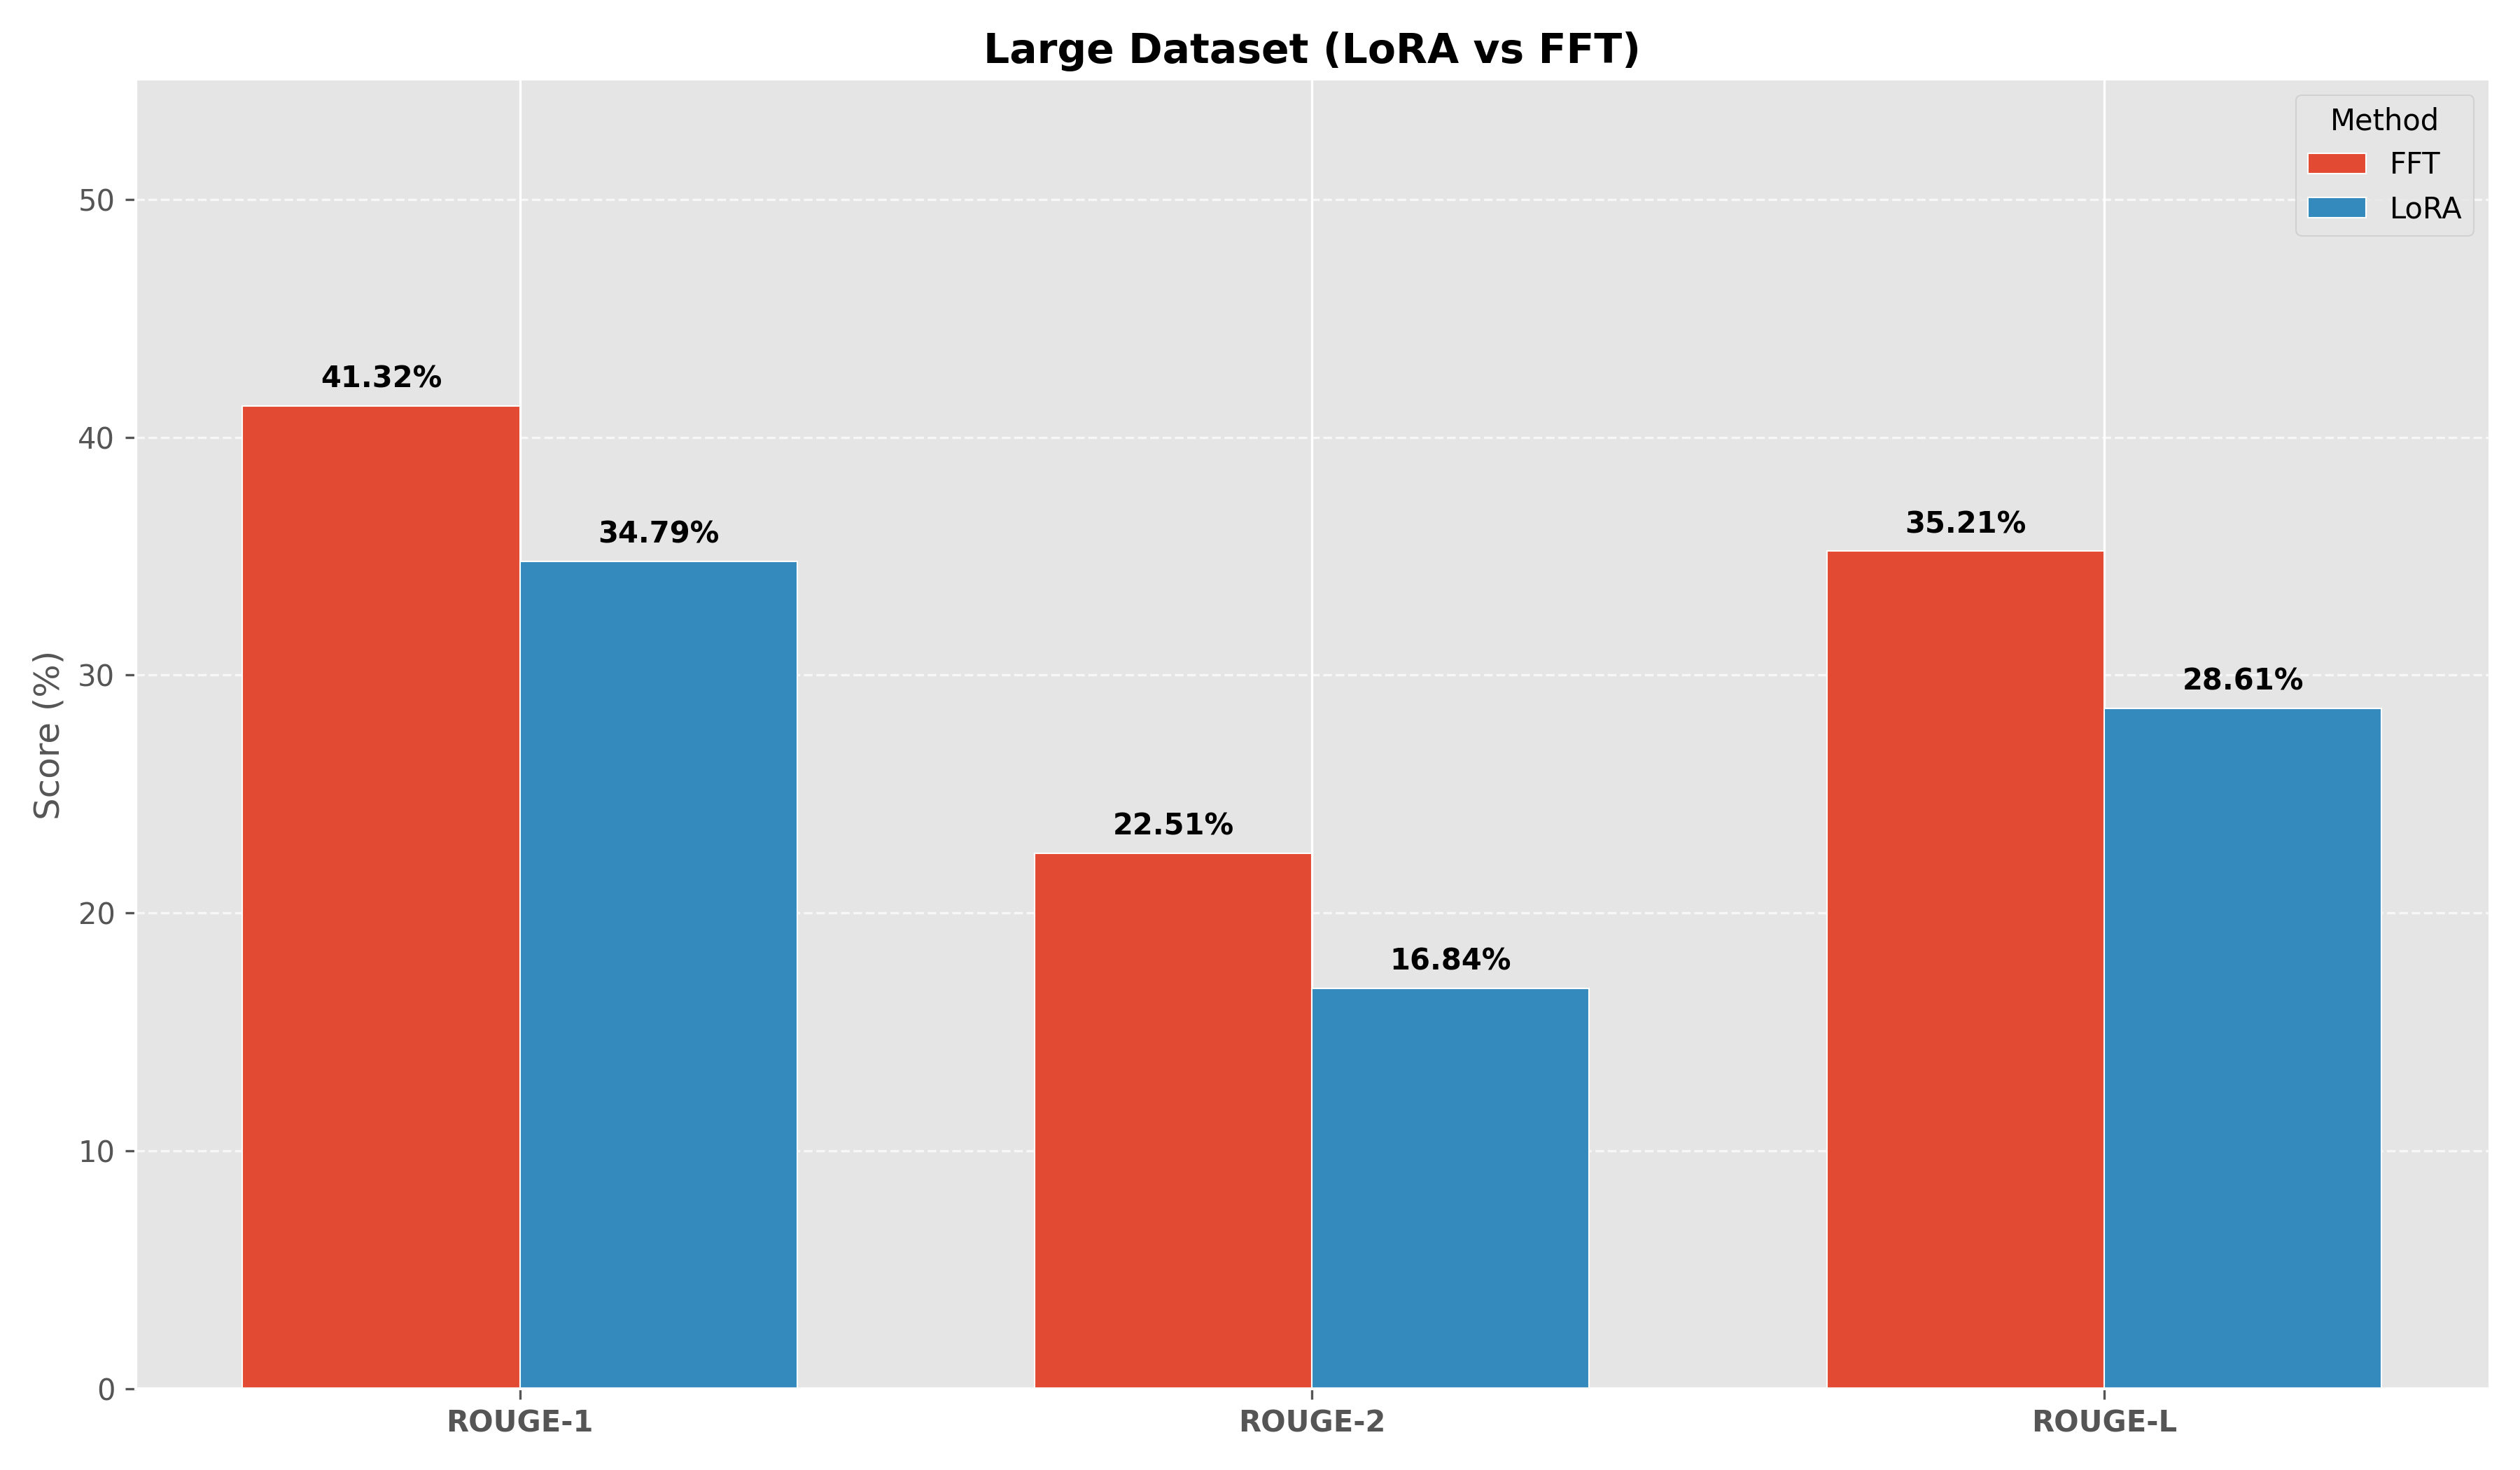
\includegraphics[width=\columnwidth]{best_comparison_own.png}
\caption{Best ROUGE scores of \textbf{Large Dataset} between LoRA (5 epochs) and FFT (1 epoch). The validation set was LREC-COLING 2024.}
\label{fig:comparisonLoRAFFTOwn}
\end{figure}

In Figure \ref{fig:comparisonLoRAFFTOwn} \& \ref{fig:comparisonLoRAFFTCSPubSum}, one can see that full fine-tuning always outperforms LoRA by a notable margin. Why this could be is discussed in the following chapter.

\begin{figure}[htbp]
\centering
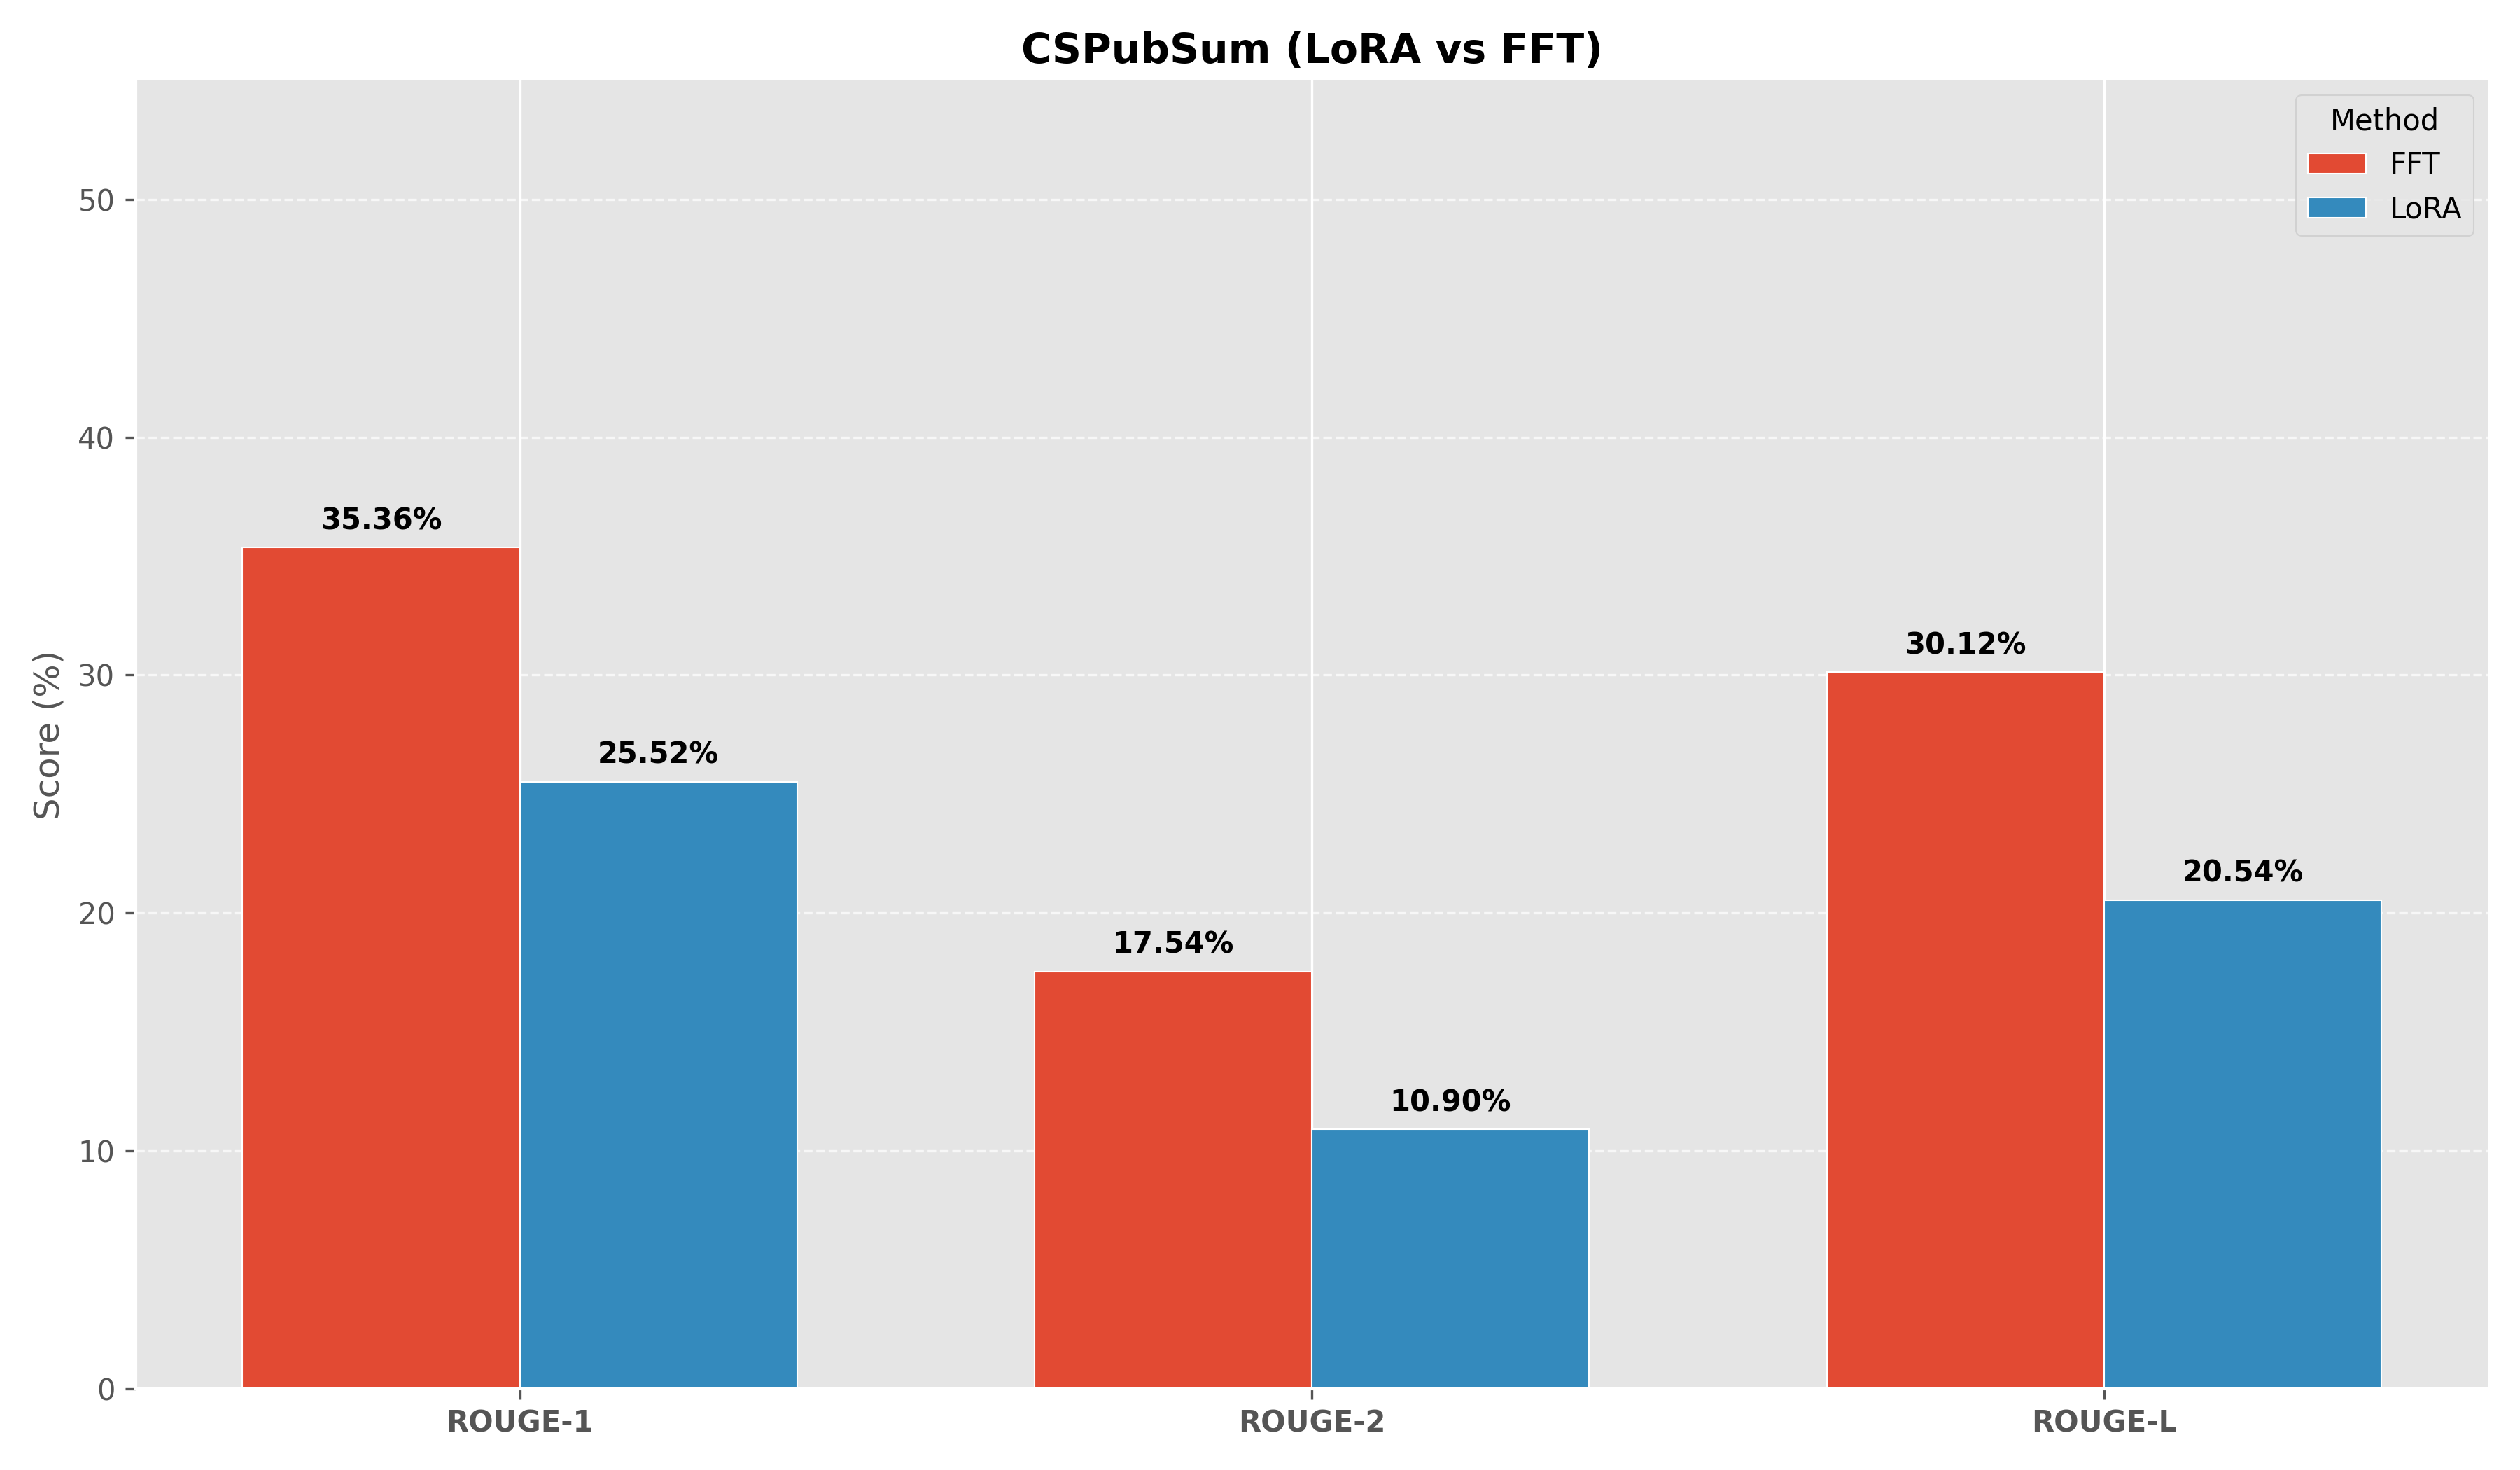
\includegraphics[width=\columnwidth]{best_comparison_CSPubSum.png}
\caption{Best ROUGE scores of \textbf{CSPubSum} between LoRA (5 epochs) and FFT (1 epoch). The validation set was LREC-COLING 2024.}
\label{fig:comparisonLoRAFFTCSPubSum}
\end{figure}

\section{Discussion}
\subsection{Dataset Scale vs. Domain Specificity}
My biggest finding is that the large diverse dataset does not always outperform the in-domain CSPubSum dataset, despite the former still containing substantially more scientific content. This suggests that, for a model as small as SmolLM-135M, learning the general task of summarizing text into a short, descriptive headline from a large and varied corpus may be too much and more confusing than learning the narrow stylistic conventions of scientific titles (underfitting). Larger models, by contrast, may be better positioned to exploit in-domain data efficiently.

\subsection{Overfitting}
A potential weakness of the large dataset experiment is the risk of overtraining. Although the diverse corpus contains over 2.4 million samples after cleaning, the title length distribution differs substantially from the LREC-COLING evaluation set, which focuses on scientific papers. During the LoRA training (5 epochs), performance was observed to plateau after the first epoch on held-out validation loss. This is consistent with a form of distribution shift: the model adapts increasingly to the style of Medium blog titles and general web content, drifting away from the scientific register expected by the benchmark.

The large-scale FFT experiment was restricted to a single epoch to avoid this degradation. Even so, it is possible that the model has not fully converged, and that a more carefully tuned learning rate schedule or earlier stopping criterion could yield further improvements.

\subsection{Impact of Generation Length}
The choice of maximum generation length (\texttt{max\_new\_tokens}) has a disproportionate effect on ROUGE scores in this setting. Restricting generation to 20 tokens approximately halved ROUGE-1 performance compared to 30 tokens. This is an artifact of the training data distribution: the large dataset contains many titles substantially longer than those in CSPubSum, so the model learns to generate longer outputs. When the generation is cut short, partially generated titles receive poor ROUGE scores.

This is a methodological weakness relative to the reference paper, which evaluates models trained on domain-matched data with more consistent title lengths. If in the future further research is done, it work should consider normalizing title length either during training by filtering for length consistency or during evaluation, using length-normalized ROUGE variants.


\subsection{LoRA vs. Full Fine-Tuning}
At this model scale, full fine-tuning outperforms LoRA by a notable margin (41.32 vs. 35.36 ROUGE-1). This is somewhat expected: with only 135M parameters, the model is small enough that full fine-tuning remains computationally feasible, and the flexibility of updating all weights allows the model to better adapt to the target task. The advantage of LoRA lies primarily in memory efficiency and faster training iteration, which becomes more relevant for larger models. At 135M parameters, the memory savings are less critical.

\subsection{Limitations}
Several limitations should be acknowledged. First, the evaluation is restricted to ROUGE scores. I could not go into detail to report the full entity-level factual consistency metrics from the reference paper, since this would extend the paper by a notable margin. However, these can be found in the appendix. 

Second, the LREC-COLING 2024 test set evaluates performance on computer science papers, but the large training dataset is heavily weighted toward general web content after the LaTeX filtering step, creating a domain mismatch that may suppress performance. 

Third, no hyperparameter search was conducted; the learning rates, batch sizes, and LoRA rank were chosen based on reasonable defaults rather than systematic optimization. 

Fourth, and most fundamentally, SmolLM-135M is a decoder-only causal model, whereas the best-performing reference models (T5, BART, PEGASUS) are encoder-decoder architectures specifically designed for conditional generation. This architectural difference may inherently disadvantage our approach for short, precise generation tasks. This can also be seen when comparing the ROUGE scores visually (Figure \ref{fig:comparisonAll}). All decoder \& encoder models dominate the benchmarks, even compared to much bigger decoder only models like the 8 billion Llama 3 model.

\begin{figure}[htbp]
\centering
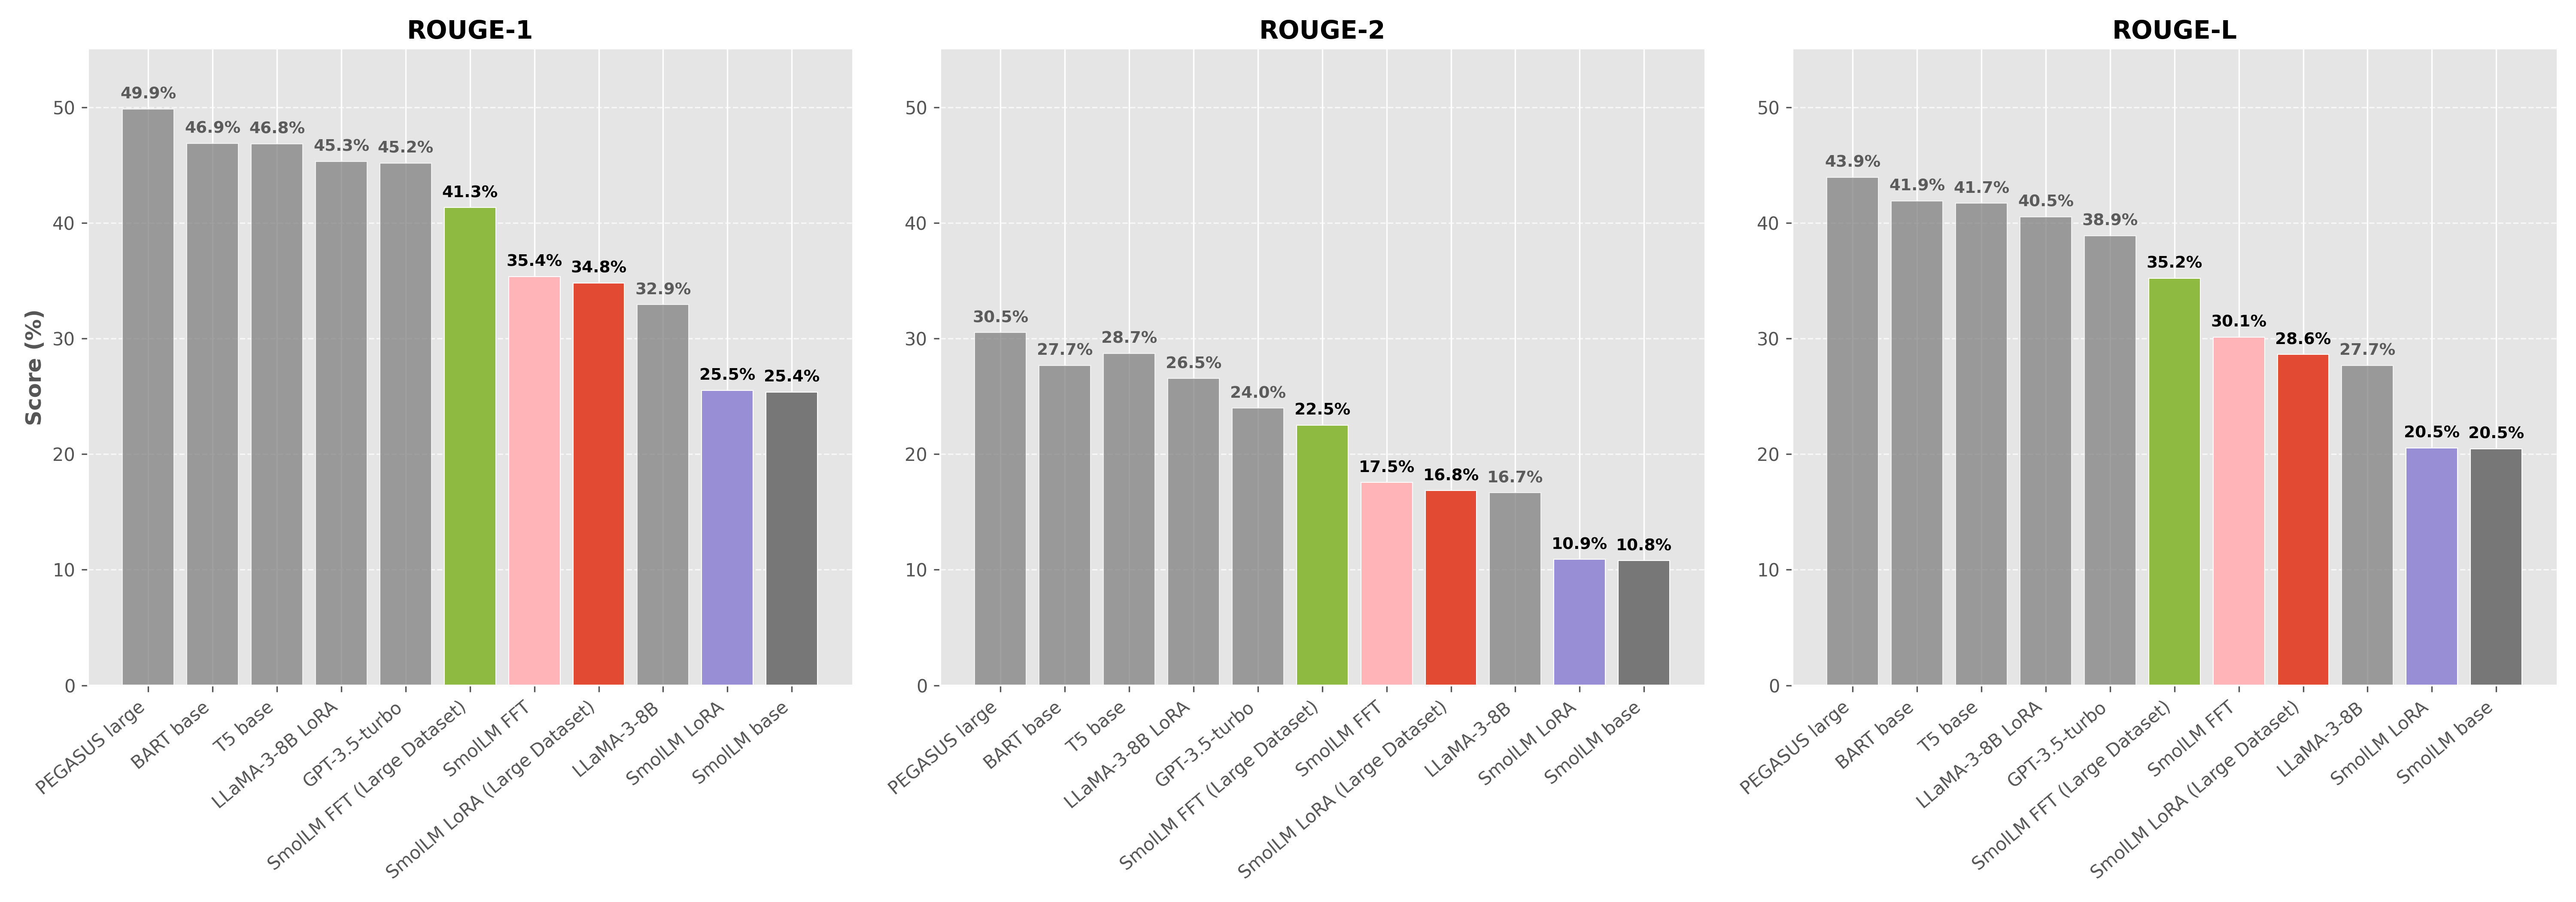
\includegraphics[width=170mm, angle=90]{best_comparison_CSPubSum_all.png}
\caption{Best ROUGE Scores of all models, compared visually. All SmolLM models are color coded.}
\label{fig:comparisonAll}
\end{figure}

\section{Practical Deployment: Title Generation in the Browser}

As a practical contribution beyond the numerical results, the LoRA adapters were merged back into the base model was converted to ONNX format using the Optimum library and subsequently deployed as a browser-based application using Transformers.js. ONNX runtime allows model inference to run entirely within the browser via WebAssembly, without requiring any API calls (apart from downloading the model into local storage once).

The pipeline for deployment is as follows: the LoRA adapter checkpoint is first merged into the base model weights, producing a standard HuggingFace model. This model is then exported to ONNX. The resulting model file, along with the tokenizer configuration, is saved and hosted on HuggingFace Hub under the identifier throvn/abstract-title-generator.
The live demo is accessible at:

https://throvn.github.io/abstract-title-generator-frontend/

Users can paste any scientific abstract (or other text) into the interface and receive a generated title directly in the browser. The model runs locally on the user's machine after the initial download.

\begin{figure}[htbp]
\centering
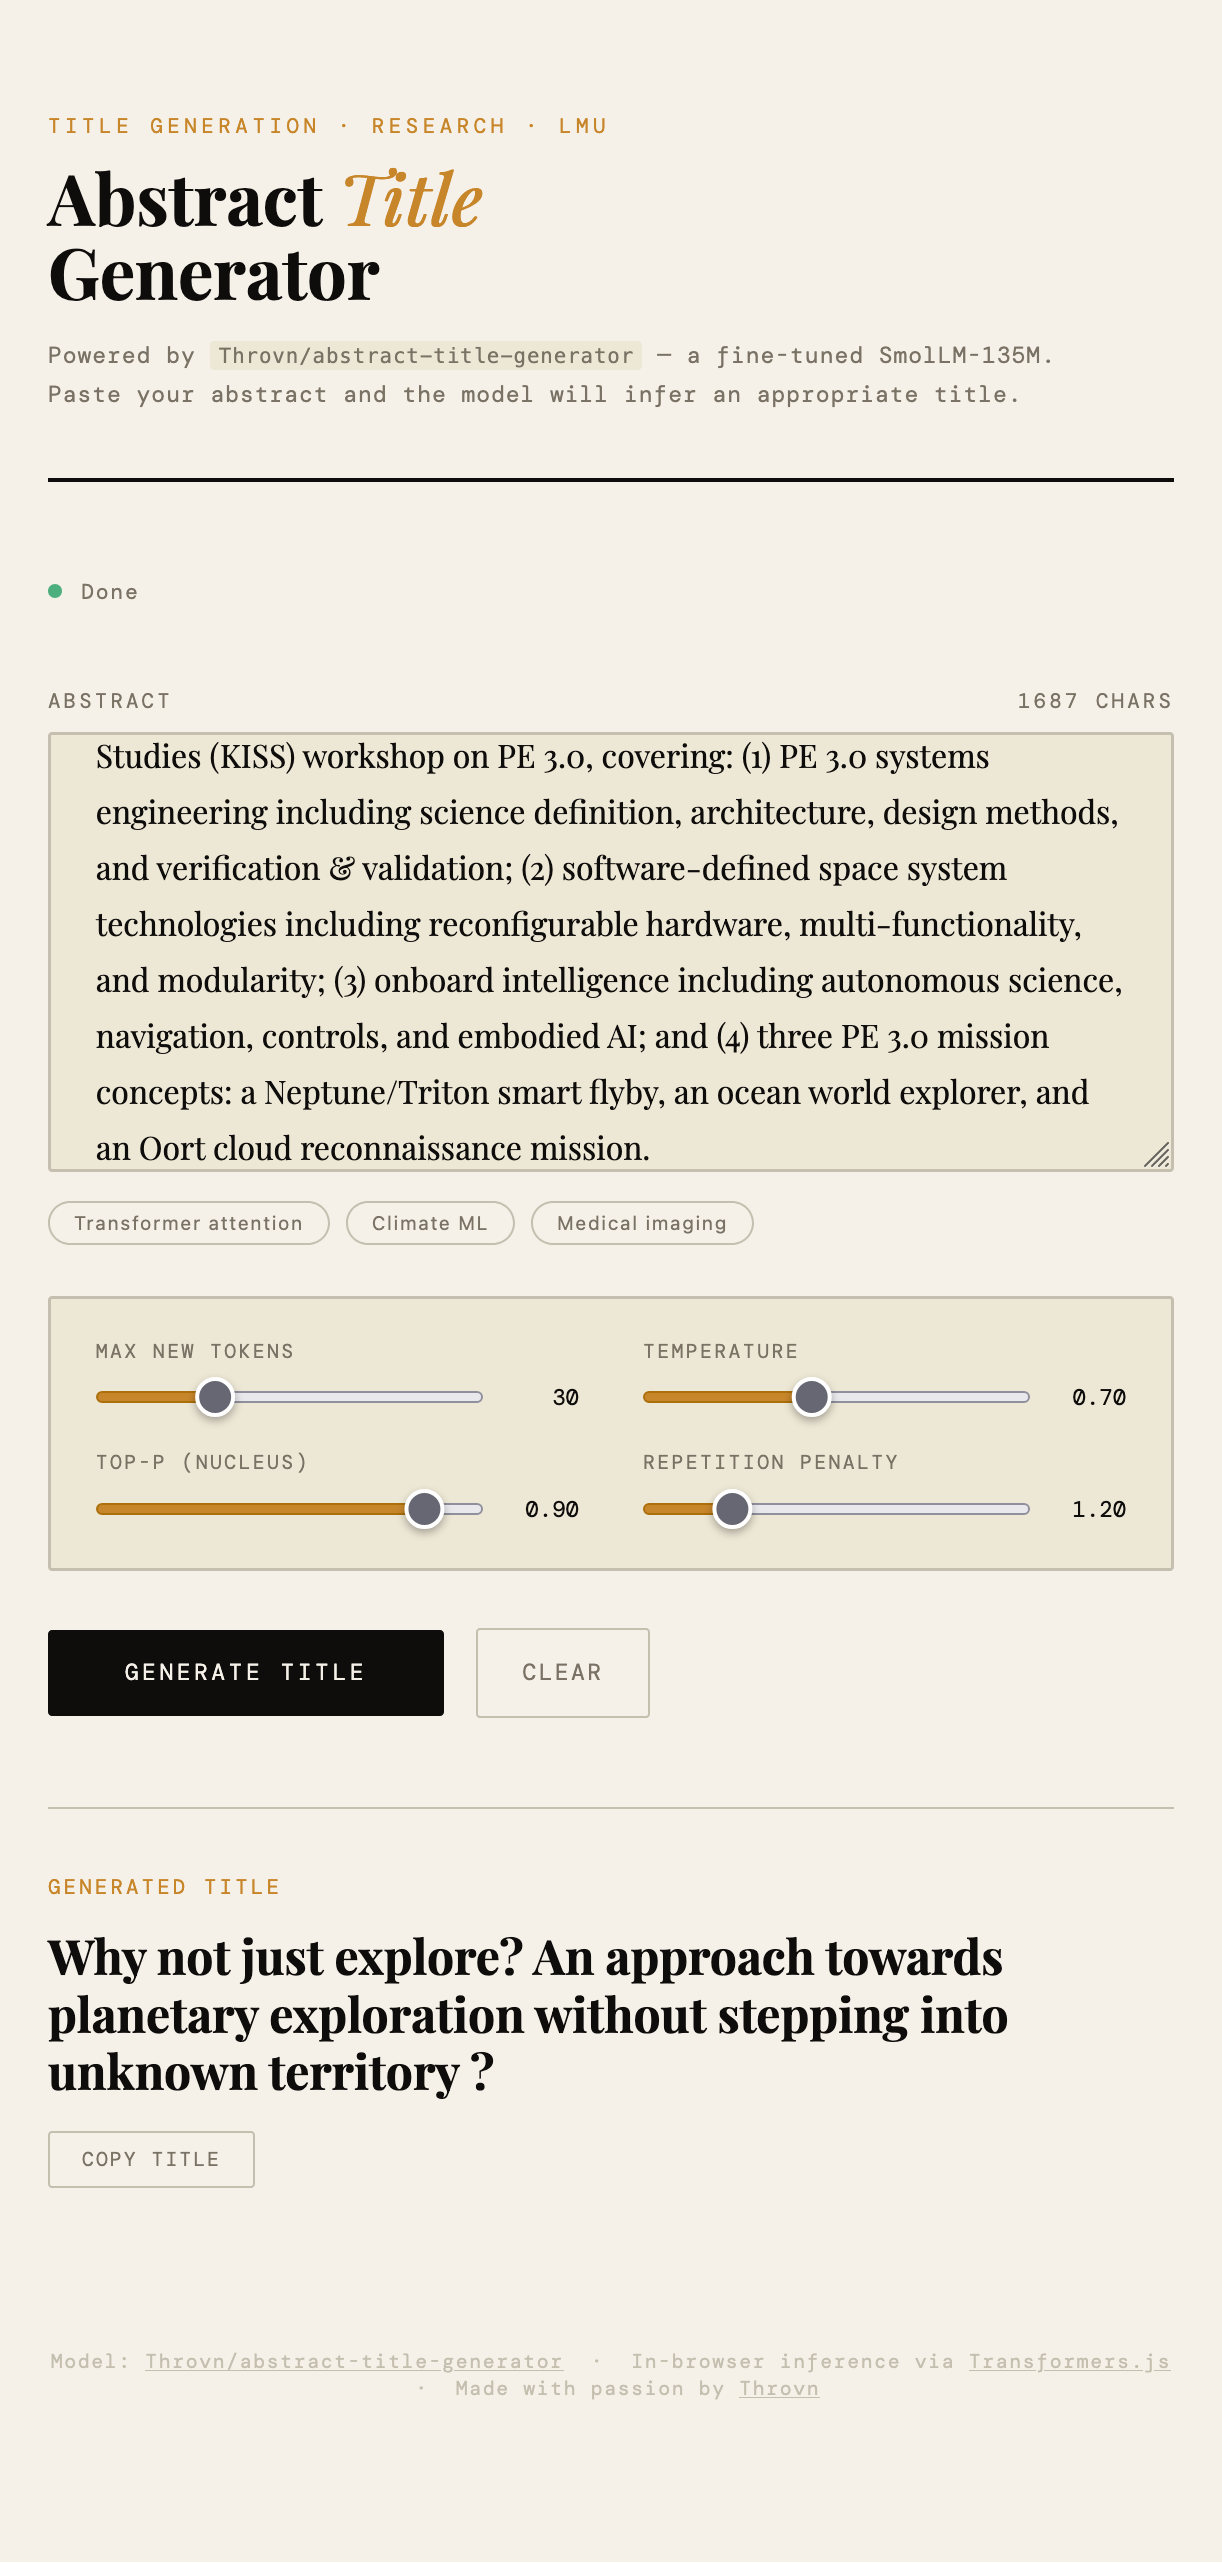
\includegraphics[width=1\columnwidth]{AbstracTitleGenerator.png}
\caption{Online hosted abstract title generator}
\label{fig}
\end{figure}

\section{Conclusion}
This work presented a partial replication and extension of the paper "Can Pre-Trained Language Models Generate Titles for Research Papers?" using SmolLM-135M, a 135-million parameter language model. I conducted experiments across two fine-tuning strategies and two dataset regimes, finding that the combination of full fine-tuning and a large diverse training corpus yields ROUGE-1/2/L scores of 41.32/22.51/35.21 on the LREC-COLING 2024 benchmark. This result is competitive with zero-shot LLaMA-3-8B and within reasonable range of fine-tuned models an order of magnitude larger (like ChatGPT-3.5-turbo).

My findings support the hypothesis that title generation, being a relatively constrained and short-form generation task, does not necessarily require large model capacity. The primary bottleneck at the 135M scale appears to be training data quality rather than scale or model size.

\section{Data \& Code}
Since the resources are too big to submit to moodle, I host them on github, kaggle, and huggingface. The resources are available here: 
\begin{itemize}
    \item  \href{https://github.com/Throvn/aaml-project}{Source Code}
    \item \href{https://www.kaggle.com/datasets/throvn/lrec-coling-2024}{LREC-COLING 2024 Dataset}
    \item \href{https://huggingface.co/Throvn/abstract-title-generator}{Finetuned LoRA Model (transformers.js compatible)}
\end{itemize}

\section{Appendix}

\begin{table}[htbp]
\caption{Factual Consistency scores for non unique entities}
\begin{center}
\begin{tabular}{|l|c|c|c|}
\hline
\textbf{Model} & \multicolumn{3}{|c|}{\textbf{NU Target Metrics}} \\
\cline{2-4}
& \textbf{\textit{Precision}} 
& \textbf{\textit{Recall}} 
& \textbf{\textit{F1}} \\
\hline
T5-base                        & 63.06 & 59.24 & 57.17 \\
BART-base                      & 64.30 & 59.21 & 57.78 \\
PEGASUS-large                  & 66.32 & 64.64 & 61.47 \\
LLaMA-3-8B$^{*}$               & 45.29 & 48.16 & 43.48 \\
LLaMA-3-8B                     & 62.18 & 55.99 & 55.19 \\
GPT-3.5-turbo                  & 60.87 & 57.66 & 55.56 \\
SmolLM-135M FFT Large Dataset  & 51.13 & 38.90 & 41.68 \\
SmolLM-135M FFT CSPubSum       & 41.53 & 35.11 & 35.75 \\
SmolLM-135M LoRA Large Dataset & 36.89 & 53.20 & 41.37 \\
SmolLM-135M LoRA CSPubSum      & 24.61 & 36.15 & 27.93 \\
\hline
\multicolumn{4}{l}{$^{*}$ Zero-shot evaluation. Metrics reported as percentages.}
\end{tabular}
\label{tab:nu_metrics}
\end{center}
\end{table}


% ================= U Metrics =================
\begin{table}[htbp]
\caption{Factual Consistency scores for unique entities}
\begin{center}
\begin{tabular}{|l|c|c|c|}
\hline
\textbf{Model} & \multicolumn{3}{|c|}{\textbf{U Target Metrics}} \\
\cline{2-4}
& \textbf{\textit{Precision}} 
& \textbf{\textit{Recall}} 
& \textbf{\textit{F1}} \\
\hline
T5-base                        & 62.80 & 58.88 & 56.87 \\
BART-base                      & 64.11 & 58.92 & 57.56 \\
PEGASUS-large                  & 66.15 & 64.30 & 61.28 \\
LLaMA-3-8B$^{*}$               & 45.02 & 47.64 & 43.13 \\
LLaMA-3-8B                     & 62.13 & 55.95 & 55.16 \\
GPT-3.5-turbo                  & 60.84 & 57.69 & 55.56 \\
SmolLM-135M FFT Large Dataset  & 51.02 & 38.70 & 41.51 \\
SmolLM-135M FFT CSPubSum       & 41.41 & 34.68 & 35.51 \\
SmolLM-135M LoRA Large Dataset & 35.95 & 46.88 & 38.79 \\
SmolLM-135M LoRA CSPubSum      & 24.18 & 34.13 & 26.98 \\
\hline
\multicolumn{4}{l}{$^{*}$ Zero-shot evaluation. Metrics reported as percentages.}
\end{tabular}
\label{tab:u_metrics}
\end{center}
\end{table}

\begin{figure}[htbp]
\centering
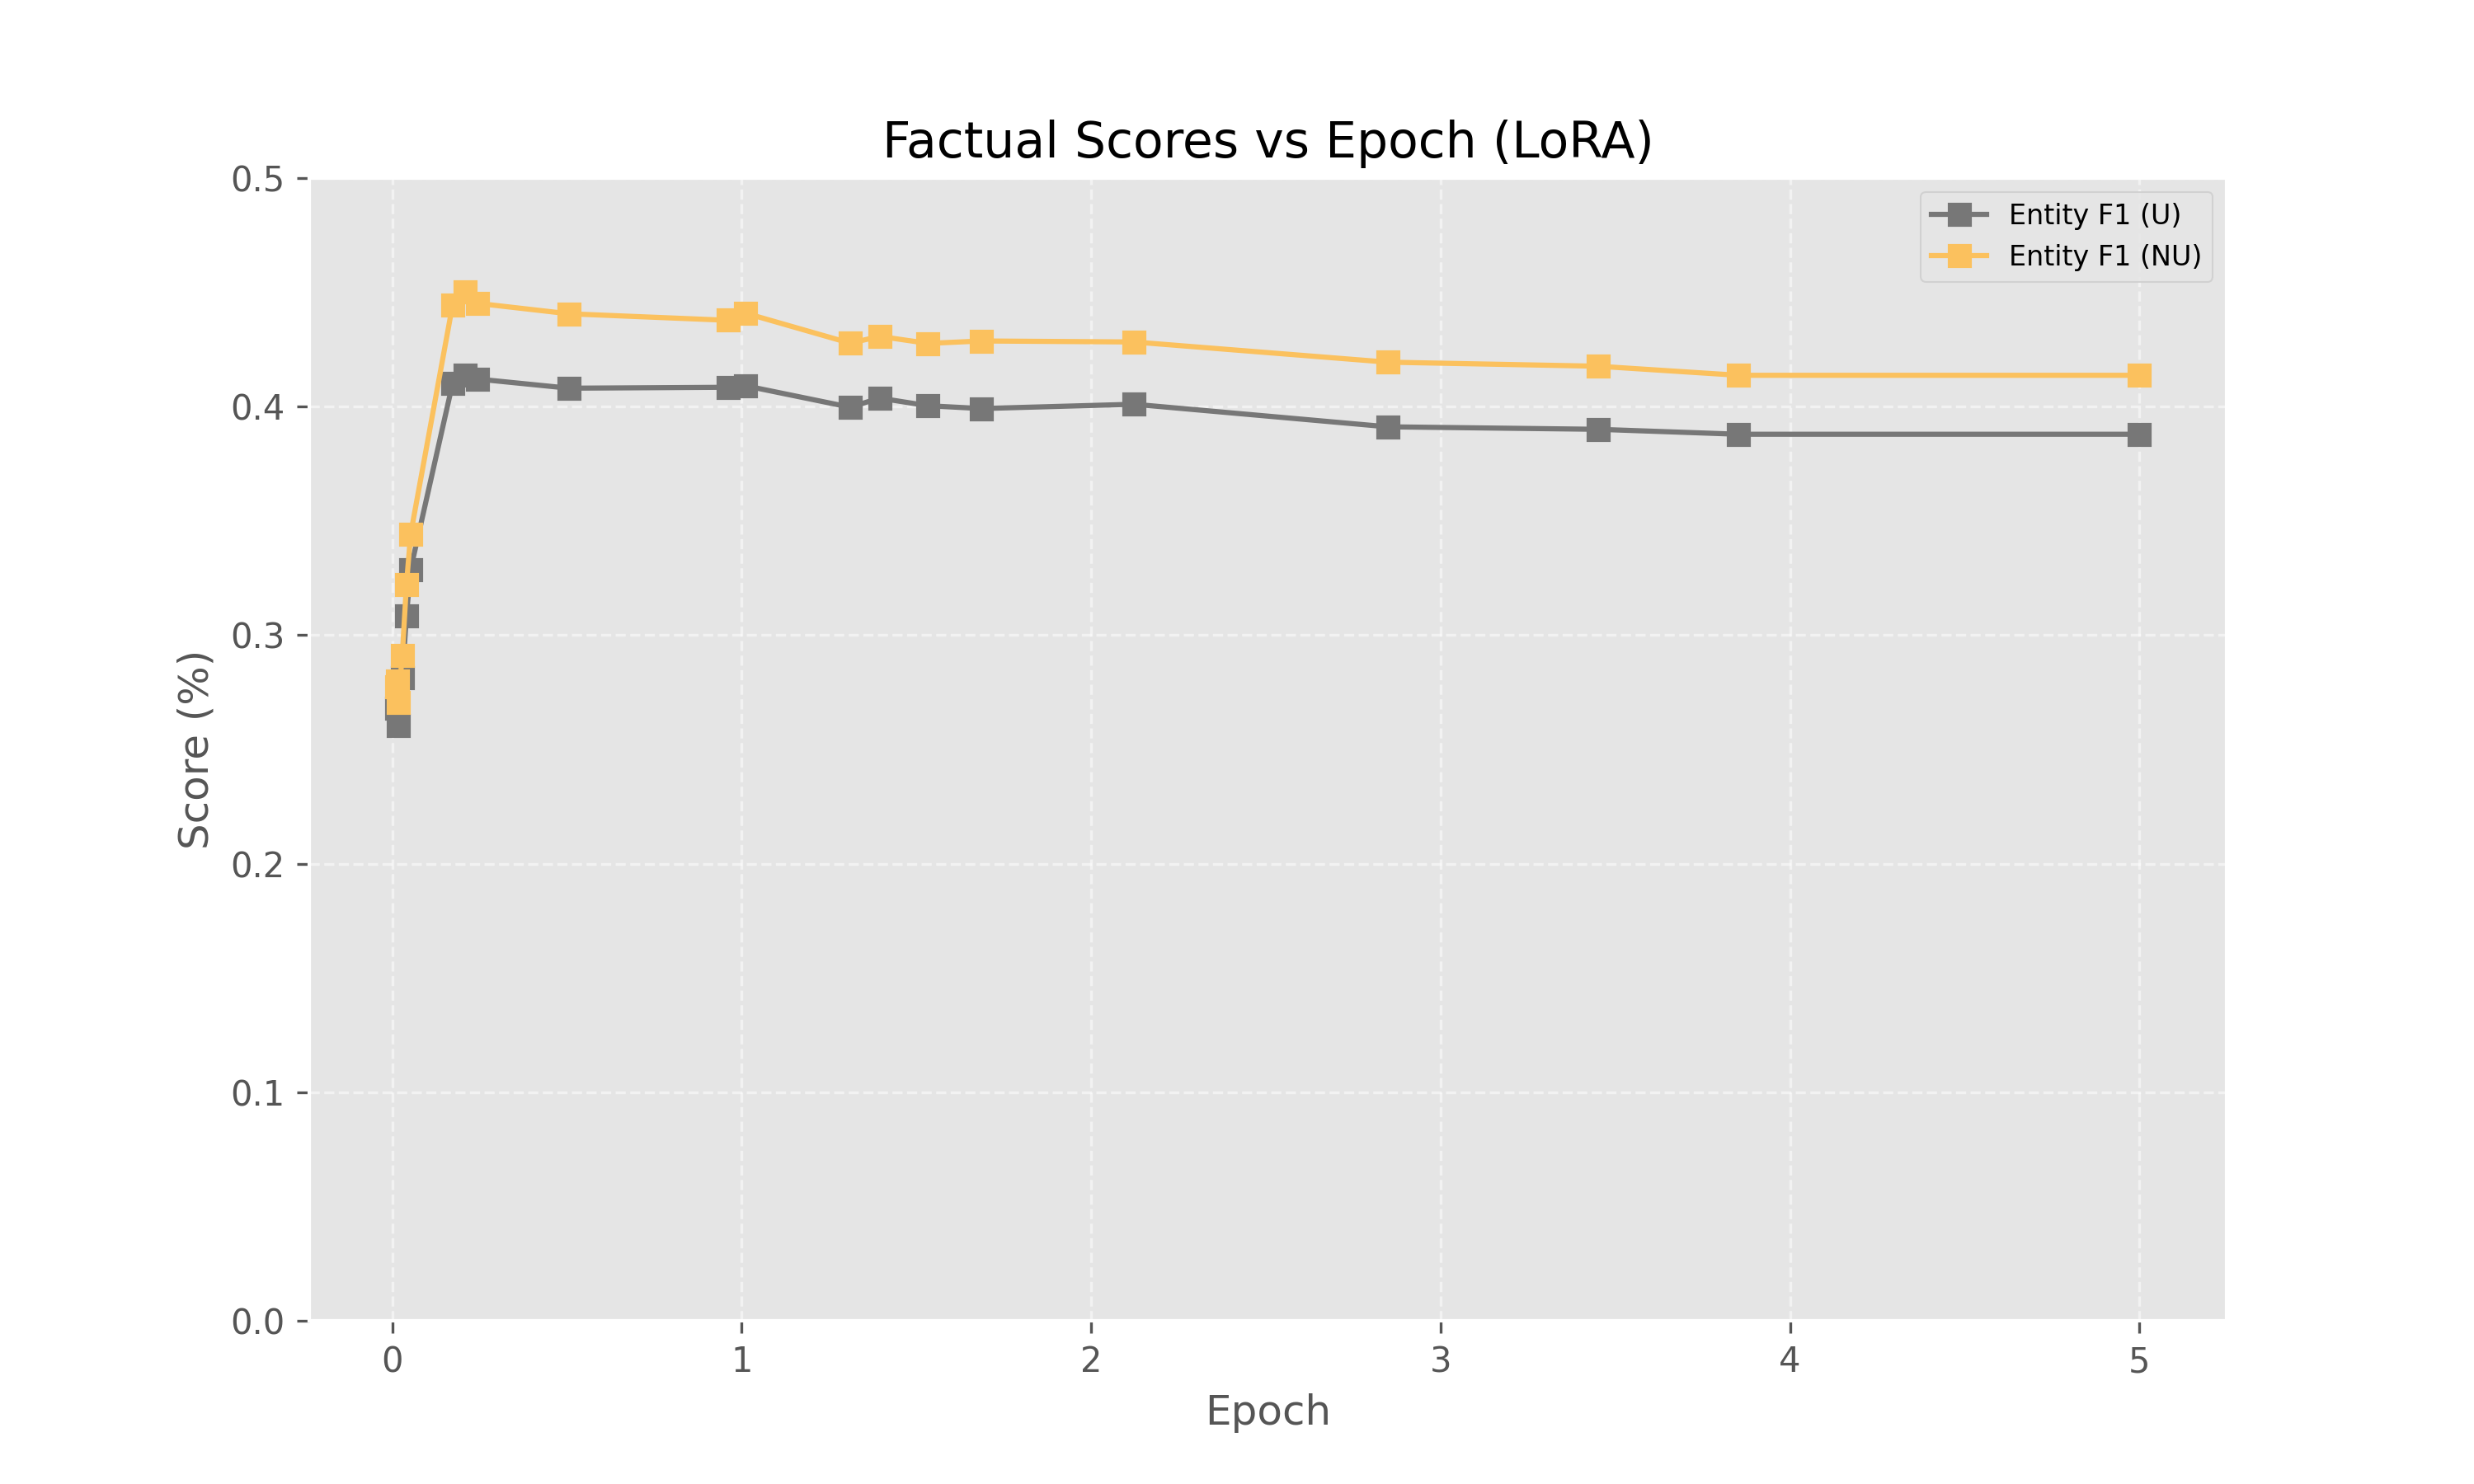
\includegraphics[width=1\columnwidth]{factual_own.png}
\caption{Online hosted abstract title generator}
\label{fig:FactualOwn}
\end{figure}

\begin{thebibliography}{00}

\bibitem{b1}
Sutskever, Ilya, Oriol Vinyals, and Quoc V. Le. "Sequence to sequence learning with neural networks." Advances in neural information processing systems 27 (2014).

\bibitem{b2}
Rehman, Tohida, Debarshi Kumar Sanyal, and Samiran Chattopadhyay. "Can pre-trained language models generate titles for research papers?." International Conference on Asian Digital Libraries. Singapore: Springer Nature Singapore, 2024.

\bibitem{b3}
Hu, Edward J., et al. 
"Lora: Low-rank adaptation of large language models." 
Iclr 1.2 (2022): 3.

\bibitem{b4}
HuggingFace,
``SmolLM - blazingly fast and remarkably powerful''
2024. [Online]. Available: https://huggingface.co/blog/smollm

\bibitem{b5}
Z. Liu, C. Zhao, F. Iandola, C. Lai, Y. Tian, I. Fedorov, Y. Xiong, E. Chang, Y. Shi, R. Krishnamoorthi, L. Lai, and V. Chandra,
``MobileLLM: Optimizing Sub-billion Parameter Language Models for On-Device Use Cases,''
\emph{arXiv preprint arXiv:2402.14905}, 2024. [Online]. Available: https://arxiv.org/abs/2402.14905

\bibitem{b6}
Hugging Face,
``cosmo2-tokenizer: Tokenizer for the training of cosmo2,''
2024. [Online]. Available: https://huggingface.co/HuggingFaceTB/cosmo2-tokenizer

\bibitem{b7}
Throvn,
``LREC-COLING 2024: Collection of datasets from the Joint International Conference on Computational Linguistics, Language Resources and Evaluation,''
2024. [Online]. Available: https://www.kaggle.com/datasets/throvn/lrec-coling-2024

\bibitem{b8}
Hugging Face,
``SmolLM-135M: A 135M-parameter small language model from the SmolLM family,''
2024. [Online]. Available: https://huggingface.co/HuggingFaceTB/SmolLM-135M

\bibitem{b9}
Hugging Face,
``PEFT (Parameter-Efficient Fine-Tuning): Documentation for efficient adaptation of large pretrained models,''
2024. [Online]. Available: https://huggingface.co/docs/peft/index

\bibitem{b10}
Lin, Chin-Yew. 
"Rouge: A package for automatic evaluation of summaries." Text summarization branches out. 2004.

\bibitem{b11}
Google LLC,
``rouge-score: Pure Python implementation of ROUGE-1.5.5,''
2019. [Online]. Available: https://pypi.org/project/rouge-score/
\end{thebibliography}
\vspace{12pt}

\end{document}
